\documentclass{ta-its}
\usepackage{hyperref} % Hyperlink pada dokumen
\usepackage{listings} % Kode sumber

\renewcommand{\lstlistingname}{Kode Sumber}


% \title{Judul Bahasa Indonesia}{Judul Bahasa Inggris}
\title{Rancang Bangun Sistem Load Balancing Menggunakan Algoritma Berbasis Konten dan Kontrol Ketersediaan Layanan}{Design and Implementasion of Load Balancing System with Content-Based Algorithm and Availability Control}{KI1502} 

% \author{Nama Lengkap}{NRP}
\author{Bahrul Halimi}{5111100014}

% \supervisorOne{Nama Pembimbing Satu}{NIP}
% \supervisorTwo{Nama Pembimbing Dua}{NIP}
\supervisorOne{Royyana Muslim Ijtihadie, S.Kom, M.Kom, PhD}{197708242006041001}
\supervisorTwo{Baskoro Adi P, S.Kom, M.Kom}{197708242006041001}

% \degree{Nama Gelar}{Bidang Studi}{Program Studi}{Jurusan}{Jurusan (English)}{Fakultas}{Fakultas Singkatan}{Fakultas (English)}
\degree{Sarjana Komputer}{Arsitektur dan Jaringan Komputer}{S1}{Teknik Informatika}{Informatics}{Teknologi Informasi}{FTIf}{Information Technology}

% \time{bulan}{tahun}
\time{Desember}{2015}

\begin{document}
    \frontmatter % Halaman dengan penomoran romawi kecil
    \maketitle
    \legalityPaper % Lembar Pengesahan
    \begin{abstrak}
    	Dokumen ini merupakan dokumen contoh penggunaan templat \LaTeX{} untuk pembuatan Buku Tugas Akhir ITS. \\
    	
    	\noindent \textbf{Kata-Kunci}: \LaTeX{}, templat, Tugas Akhir, ITS.
	\end{abstrak}
   \begin{abstract}
    	Dokumen ini merupakan dokumen contoh penggunaan templat \LaTeX{} untuk pembuatan Buku Tugas Akhir ITS. \\
    	
    	\noindent \textbf{Kata-Kunci}: \LaTeX{}, templat, Tugas Akhir, ITS.
	\end{abstract}
    \chapter{Kata Pengantar}
        \textbf{Om Swastyastu}

        Puji syukur penulis haturkan kepada Ida Sang Hyang Widhi Wasa, Tuhan Yang Maha Esa karena atas \emph{asungkertha wara nugraha} beliau, penulis dapat menyelesaikan sebuah dokumentasi cara pembuatan Buku Tugas Akhir Sarjana menggunakan \LaTeX{} untuk Institut Teknologi Sepuluh Nopember, Surabaya. Dokumentasi ini diharapkan dapat membantu rekan-rekan mahasiswa S1 yang menempuh semester terakhir dengan membuat buku Tugas Akhir menggunaan sistem \emph{typesetting} \LaTeX{} yang terbukti handal dan lumrah digunakan di bidang penelitian sains dan teknik. Dokumentasi ini dibuat menggunakan templat yang penulis buat sendiri (pada berkas \texttt{ta-its.cls}) sehingga nantinya bisa digunakan kembali sehingga pembuatan buku bisa lebih dipermudah.

        Penulis menerima kritik dan saran mengenai pengembangan templat ini agar bisa menjadi lebih baik dan bisa menjadi standar \emph{de-facto} dan \emph{de-jure} dalam penulisan buku TA di seluruh civitas akademika ITS. Penulis dapat dihubungi melalui surel: \texttt{initrunlevel0@gmail.com}.

        Sekian dan Terima Kasih.
        \noindent \textbf{Om Santhi Santhi Santhi Om}

        \cleardoublepage % Mengisi penanda halaman genap yang kosong

    \tableofcontents % Daftar isi
    \listoftables % Daftar tabel
    \listoffigures % Daftar figur/gambar

\mainmatter % Halaman utama, dengan judul BAB X, nomor halaman penomoran arab
    \chapter{PENDAHULUAN}
        Pada bab ini akan dipaparkan mengenai garis besar Tugas Akhir yang meliputi latar belakang, tujuan, rumusan dam batasan permasalahan, metodologi pembuatan Tugas Akhir, dan sistematika penulisan.

        \section{Latar Belakang}
            Semakin berkembangnya internet di masyarakat membuat penggunaan aplikasi berbasis web semakin diminati. Pengguna aplikasi berbasis web ini dapat dijumpai diberbagai aktivitas harian masyarakat, diantaranya bank \emph{online}, \emph{e-commerce}, reservasi tempat secara \emph{online}, bahkan pendaftaran peserta didik baru secara \emph{online}. Hal ini membuat penyedia layanan aplikasi berbasis web harus menyediakan servis yang layak sehingga aplikasi tetap berjalan dengan baik walaupun pengguna semakin bertambah.\\
			\indent Terjadinya \emph{bottleneck} (penumpukan permintaan) menjadi tantangan tersendiri ketika pengembang tidak memperhatikan sumber dayanya dan berujung pada gagalnya permintaan pengguna [1]. Muncul gagasan awal dengan penggunaan kelompok server yang akan menangani permintaan ini. Kelompok server ini akan secara bergantian melayani setiap permintaan terhadap aplikasi berbasis web ini. Dengan adanya tugas bergantian ini dibutuhkan sebuah komputer yang bertugas membagi beban kerja kelompok server. Komputer ini biasa disebut pembagi muat atau \emph{load balance}. Sistem kerja dari \emph{load balancer} ini menggunakan sebuah algoritma yang sudah ditanam untuk kemudian digunakan untuk memilih komputer mana yang harus melayani permintaan pengguna. \\
			\indent Di sisi lain sebuah aplikasi berbasis web memiliki dua jenis halaman yang mungkin di akses. Yang pertama adalah halaman berisi informasi, baik hasil \emph{query} basis data maupun tidak, selanjutnya disebut halaman informasi dan yang kedua adalah halaman yang digunakan untuk mengirimkan data ke server, dalam hal ini berupa form pengisian informasi, selanjutnya disebut halaman daftar. \\
			\indent Dua jenis halaman ini memiliki kebutuhan yang berbeda. Untuk halaman informasi, pengguna mengharapkan akses yang cepat sedangkan untuk halaman daftar, pengguna mengharapkan data yang dimasukkan dapat diproses dengan aman. Padahal di dalam penggunaan algoritma sebelumnya dan dengan teknologi yang ada, \emph{load balancer} tidak dapat memisahkan dua jenis permintaan ini. Algoritma yang ada sebelumnya hanya memisahkan banyak permintaan sesuai dengan ketersediaan server melayani pengguna. Padahal ketika proses pemasukkan data di dalam halaman daftar, seharusnya bisa digunakan untuk melayani permintaan pada halaman informasi. \\
			\indent Muncullah gagasan lain mengenai pengelompokkan permintaan berdasarkan konten yang diinginkan oleh pengguna. Pengelompokkan ini didasarkan pada dua halaman sebelumnya, yakni halaman informasi dan halaman daftar. Tujuannya untuk mengatur penggunaan sumber daya yang digunakan. Dua kelompok server terpisah akan melayani masing-masing permintaan yang berbeda. Dengan permintaan satu tipe dalam satu kelompok server, membuat kerja server menjadi lebih terpusat dan mengurangi beban yang besar. \\
			\indent Berbeda dengan yang terjadi saat ini, sebuah server atau bahkan dalam sebuah kelompok server, harus melayani berbagai bentuk permintaan dari pengguna, sehingga menyebabkan beban kerja server meningkat. Bahkan waktu dalam penyelesaian suatu permintaan tidak dapat diukur dalam satuan waktu yang sama karena berbedanya bentuk permintaan pengguna. \\
			\indent Sementara itu di dalam kelompok server yang bekerja bergantian melayani permintaan, ada kalanya sebuah server mengalami gangguan dan sama sekali tidak dapat melayani setiap permintaan pengguna. Padahal setiap permintaan yang ada masih diteruskan oleh load balancer pada server tersebut. Tidak adanya mekanisme untuk memindahkan permintaan dari server mati ke server yang masih aktif membuat akses ke sebuah web menjadi tidak maksimal.
			Oleh karena itu dibangunlah sistem ini. Dengan adanya sistem load balancing menggunakan algoritma berbasis konten yang memisahkan antara halaman informasi dan halaman daftar diharapkan dapat meningkatkan jumlah pengguna suatu halaman web dengan banyaknya bentuk permintaan dari pengguna.

            
        \section{Rumusan Masalah}
			Berikut beberapa hal yang menjadi rumusan masalah dalam tugas akhir ini:
			\begin{enumerate}
			\item Bagaimana membagi beban kerja server berdasarkan konten permintaan pengguna ?
			\item Bagaimana menentukan pengelompokkan server berdasarkan konten permintaan pengguna ?
			\item Bagaimana meningkatkan jumlah pengakses pada halaman informasi dengan terpisahnya akses antara halaman informasi dan halaman daftar ?
			\item Bagaimana menjaga pengguna tetap dilayani kelompok ser-ver yang tersedia hingga permintaan selesai ?
			\end{enumerate}

        \section{Batasan Masalah}
			Dari permasalahan yang telah diuraikan di atas, terdapat beberapa batasan masalah pada tugas akhir ini, yaitu:
			\begin{enumerate}
			\item Konten permintaan pengguna dilihat dari URL yang diakses.
			\item Pendefinisian kelompok konten permintaan pengguna dilakukan manual oleh manusia.
			\item Sistem pembagi beban kerja diimplementasikan untuk aplikasi berbasis web.
			\item Kelompok server yang bekerja dibedakan dengan besar memori yang digunakan.
			\end{enumerate}

        \section{Tujuan}
			Tugas akhir dibuat dengan beberapa tujuan. Berikut beberapa tujuan dari pembuatan tugas akhir:
			\begin{enumerate}
			\item Mampu mengategorikan permintaan pengguna terhadap suatu web berdasarkan halaman yang diakses pengguna.
			\item Mampu melayani banyaknya permintaan pengguna dengan mengandalkan pengelompokan komputer.
			\item Mampu meningkatkan jumlah pengakses yang dilayani dengan berhasil oleh aplikasi dibandingkan dengan akses tanpa pemisahan jenis halaman yang diakses.
			\end{enumerate}

        \section{Manfaat}
			Dengan dibangunnya \emph{load balancer} ini diharapkan jumlah pengakses yang mampu dilayani oleh kelompok server untuk halaman informasi menjadi lebih banyak dibandingkan dengan penggunaan algoritma dan teknologi \emph{load balancing} yang sudah ada.

   \chapter{LANDASAN TEORI}
        \section{Algoritma Berbasis Konten}
			Munculnya algoritma ini didasarkan pada beberapa jenis permintaan pengguna yang mengakses suatu halaman web. Sebuah server melayani berbagai jenis permintaan akan memberikan waktu balasan yang beragam pula. Hal ini akan meningkatkan beban kerja server. \\
			\indent Dengan adanya pemisahan permintaan pengguna berdasarkan konten, kelompok server akan melayani setiap permintaan yang memang ditujukan untuknya server tersebut. Bentuk permintaan akan selalu sama sehingga waktu untuk melayani permintaan menjadi sama dan lebih terkontrol. Beban kerja server akan lebih ringan dengan adanya pembagian beban berdasarkan algoritma ini. [1]

        \section{Node JS}
			Merupakan sebuah platform yang dibangun di atas Chrome's JavaScript runtime dengan teknologi V8 yang mendukung proses server yang bersifat long-running. Tidak seperti platform modern yang mengandalkan multithreading, NodeJS memilih menggunakan asynchronous I/O eventing. Karena inilah NodeJS mampu bekerja dengan konsumsi memori rendah. [2] [3]
			
			Teknologi yang tidak memanfaatkan multi-thread ini memudahkan pengembang yang terkadang kesulitan mengatur sumberdaya yang digunakan thread. Karena tidak mungkin ada sumberdaya yang terkunci karena thread yang berjalan. Akhirnya banyak yang memanfaatkan kemampuan dasar NodeJS sebagai web server.
			
			\begin{figure}[h] % h = pasti berada di bawah teks yang ada di atas
				\centering
				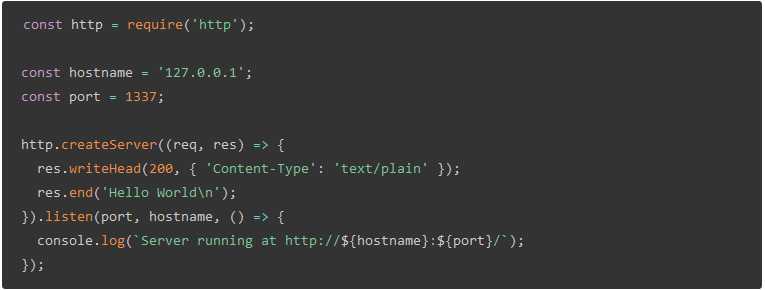
\includegraphics[width=\linewidth]{contoh_img/contoh_nodejs}
				\caption{Contoh Penggunaan NodeJS sebagai Web Server}
				\label{contohNodeJS}
			\end{figure}
			
			
			Dengan adanya callback untuk setiap penggunaan fungsi, memungkinkan setiap pemanggilan fungsi yang tidak menghasilkan apapun, NodeJS akan \textit{sleep}

        \section{Angular JS}
			Angular JS membantu dalam pembangunan halaman HTML menjadi lebih dinamis. Merupakan sebuah kumpulan alat bantu yang mampu bekerja baik dengan pustaka lainnya. Setiap fitur dapat dimodifikasi sesuai dengan kebutuhan aplikasi. Menjadi salah satu kerangka kerja yang memfasilitasi pembangunan aplikasi kompleks yang terorganisir dan mudah dirawat. Angular JS lebih dikenal pada kemampuannya melayani sebuah situs web yang menggunakan halaman tunggal untuk penyajian data yang beragam. [4][5]
			
			\begin{figure}[h] % h = pasti berada di bawah teks yang ada di atas
				\centering
				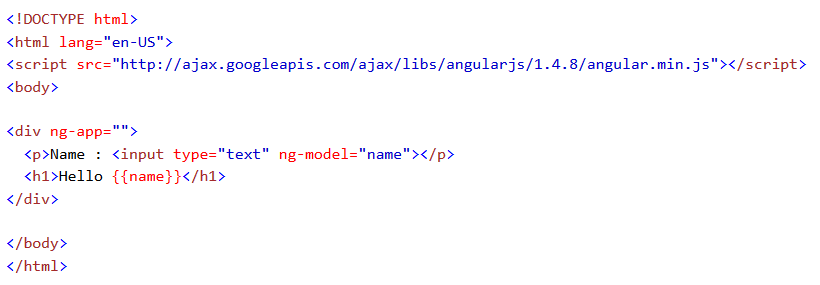
\includegraphics[width=\linewidth]{contoh_img/contoh_angular}
				\caption{Contoh Penggunaan Angular JS pada Halaman Sederhana}
				\label{contohAngularJS}
			\end{figure}

			Dengan menggunakan berkas JavaScript Angular yang didapatkan dari CDN (\textit{Content Delivery Network}) atau media lain, pengembang dapat dengan mudah menggunakan fitur yang ditawarkan Angular JS.
			
		\section{MongoDB}
			Merupakan salah satu NoSQL (Not only SQL) terkenal yang dirancang untuk mengelola polimorfik, obyek, dan struktur data yang terus berkembang. MongoDB adalah basis data open-source yang memungkinan mengubah skema dengan cepat sementara fungsi yang diharapkan dari basis data tradisional masih berjalan. [6] [7]
			
			\begin{figure}[h] % h = pasti berada di bawah teks yang ada di atas
				\centering
				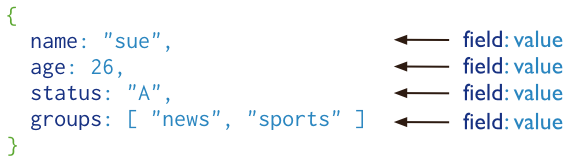
\includegraphics[width=\linewidth]{contoh_img/contoh_mongodb}
				\caption{Contoh Bentuk Penyimpanan Data MongoDB}
				\label{contohMongoDB}
			\end{figure}
			
			Model penyimpanan yang menyerupai JSON membuat pengguna dapat dengan mudah mengakses dan mengubah data yang ada. Karena penyimpanannya yang menyerupai JSON, membuat struktur penyimpanan dapat berubah sewaktu-waktu tanpa mengubah konfigurasi sebelumnya.
		
		\section{Apache JMeter}
			Menjadi salah satu alat bantu untuk melakukan tes muat dan mengukur performa aplikasi, salah satunya berbasis web. Mampu melakukan pengujian pada berbagai protokol diantaranya Web, FTP, basis data, Mail (SMTP, POP3, IMAP), serta MongoDB. [8]
			
			\begin{figure}[h] % h = pasti berada di bawah teks yang ada di atas
				\centering
				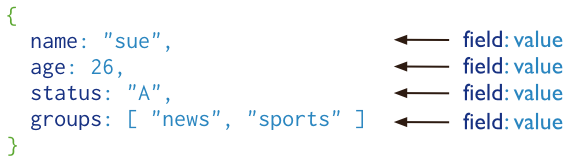
\includegraphics[width=\linewidth]{contoh_img/contoh_mongodb}
				\caption{Contoh Bentuk Penyimpanan Data MongoDB}
				\label{contohMongoDB}
			\end{figure}
			
			Apache JMeter berbasis Java. Cara kerjanya yang menyerupai sebuah browser, karena desain awal memang ditujukan untuk menguji aplikasi berbasis web, mampu mengakses halaman website yang memiliki sumber daya statis maupun dinamis. Namun ada beberapa fitur browser yang tidak ditiru oleh Apache JMeter.


    \chapter{DESAIN DAN PERANCANGAN}
	    Pada bab ini dibahas mengenai analisis dan perancangan sistem.
	    
	    \section{Kasus Penggunaan}
		    Terdapat dua aktor dengan masing-masing tiga aktivitas dalam sistem yang digambarkan pada Gambar \ref{gambarDiagramKasusPenggunaan}.
		    
		    \begin{figure}[h] % h = pasti berada di bawah teks yang ada di atas
		    	\centering
		    	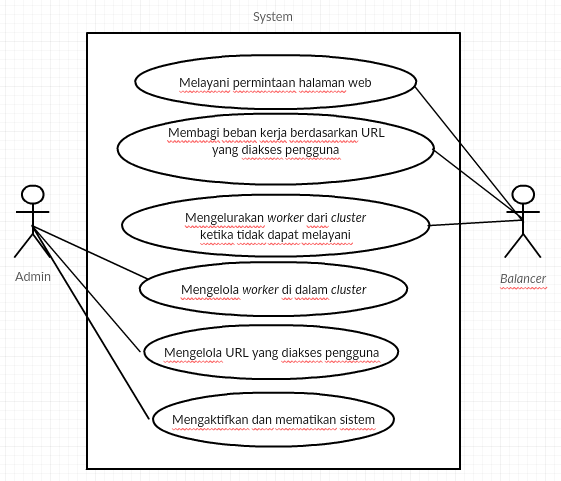
\includegraphics[width=\linewidth]{contoh_img/usecase}
		    	\caption{Digram Kasus Penggunaan}
		    	\label{gambarDiagramKasusPenggunaan}
		    \end{figure}
		    
		    Digram kasus penggunaan pada Gambar \ref{gambarDiagramKasusPenggunaan} dideskripsikan masing-masing pada Tabel \ref{tabelKodeKasusPenggunaan}.
		    \begin{ltabulary}{|L|L|L|} % L = Rata kiri untuk setiap kolom, | = garis batas vertikal.
		    	
		    	% Kepala tabel, berulang di setiap halaman
		    	\caption{Daftar Kode Kasus Penggunaan} \label{tabelKodeKasusPenggunaan} \\
		    	\hline
		    	\textbf{Kode Kasus Penggunaan} & \textbf{Nama Kasus Penggunaan} & \textbf{Keterangan} \\ \hline
		    	
		    	\endhead
		    	\endfoot
		    	\endlastfoot
		    	
		    	% Isi Tabel
		    	UC-0001 & Melayani permintaan halaman web & Setiap permintaan halaman web akan mengarah ke sistem dan \textit{balancer} akan melayani dengan cara meneruskan permintaan ke \textit{worker} dan mengeruskan balasan ke pengguna \\ \hline
		    	UC-0002 & Membagi beban kerja berdasarkan URL yang diakses pengguna & Dibelakang sistem terdapat beberapa \textit{worker} yang bekerja melayani permintaan terusan dari sistem, di sini lah \textit{balancer} membagi beban kerja tersebut \\ \hline
		    	UC-0003 & Mengeluarkan \textit{worker} dari \textit{cluster} ketika tidak dapat melayani & Jika terdapat \textit{worker} yang tidak dapat melayani permintaan, \textit{balancer} akan mengeluarkan sementara dari tugas melayani hingga \textit{worker} mampu memberikan layanan \\ \hline
		    	UC-0004 & Mengelola \textit{worker} di dalam \textit{cluster} & Admin dapat menambahkan dan mengurangi \textit{worker} di dalam daftar \textit{cluster} \\ \hline
		    	UC-0005 & Mengelola URL yang diakses pengguna & Admin dapat menambahkan dan mengurangi daftar URL ke dalam sistem \\ \hline
		    	UC-0006 & Mengaktifkan dan mematikan sistem & Admin memiliki kendali atas aktif dan tidaknya sistem \\ \hline
		    	
		    \end{ltabulary}
		    
		\section{Arsitektur Sistem}
			Pada sub-bab ini, dibahas mengenai tahap analisis dan kebutuhan bisnis dan desain dari sistem yang akan dibangun.
	    
		    \subsection{Desain Umum Sistem}
			    Sistem load balancing yang akan dibangun menggunakan teknologi Node JS dengan JavaScript sebagai bahasa pemrograman. Sistem ini akan berjalan pada port 80 dan menjadi target utama ketika pengguna akan menggunakan aplikasi berbasis web yang dikembangkan dengan menggunakan load balancer ini. Akan terdapat beberapa komputer pembantu, selanjutnya disebut \textit{worker}, yang menerima perintah untuk melayani permintaan halaman website dari load balancer. \textit{Worker} akan digolongkan menjadi dua cluster untuk melayani permintaan sesuai dengan URL yang diakses pengguna. Di sinilah algoritma berbasis konten diterapkan. Secara visual, desain sistem secara umum digambarkan pada Gambar \ref{gambarSistem}.
			    
			    \begin{figure}[h] % h = pasti berada di bawah teks yang ada di atas
			    	\centering
			    	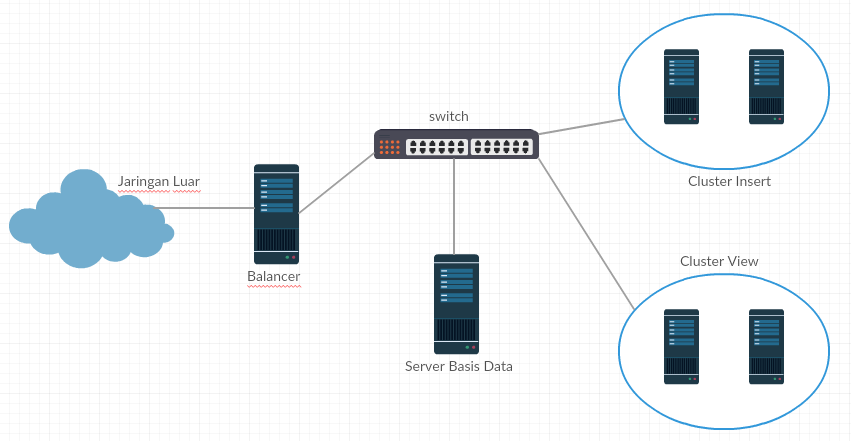
\includegraphics[width=\linewidth]{contoh_img/sistem}
			    	\caption{Desain Sistem Secara Umum}
			    	\label{gambarSistem}
			    \end{figure}
			    
			    Load balancer memiliki daftar worker dan URL yang akan digunakan dalam operasional load balancing. Untuk memudahkan administrator sistem dalam mengkonfigurasikan worker dan menambahkan daftar URL yang ada, disediakan sebuah halaman admin yang berjalan pada port 3000. Selain dengan halaman admin ini, administrator sistem sudah dibantu untuk mengeluarkan worker yang tidak aktif dari pekerjaannya dalam proses load balancing oleh sistem secara otomatis dalam rentang waktu tertentu.
			    
			    
			    
			
			\subsection{Desain Rinci Balancer}
			    \textit{Balancer} berperan penting dalam sistem. Setiap permintaan yang masuk ke dalam sistem akan diolah oleh balancer dan dikembalikan ke pengguna setelah mendapat balasan dari \textit{worker}. Ada beberapa aplikasi yang sudah menyediakan fitur \textit{balancing}, namun dalam Tugas Akhir ini digunakan NodeJS dan MongoDB untuk membangun fitur \textit{balancing}. Diagram arsitektur Balancer tertera pada Gambar \ref{gambarArsitekturBalancer} dan diagram proses pengguna mengakses halaman web tertera pada Gambar \ref{gambarKerjaBalancer}. 
			    
			    \begin{figure}[] % h = pasti berada di bawah teks yang ada di atas
			    	\centering
			    	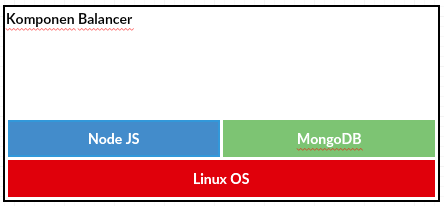
\includegraphics[width=\linewidth]{contoh_img/kompbalancer}
			    	\caption{Desain Arsitektur Balancer}
			    	\label{gambarArsitekturBalancer}
			    \end{figure}
			    
			    NodeJS akan menyediakan servis web yang akan menangkap setiap permintaan pengguna. Sebelum diteruskan ke \textit{worker}, \textit{balancer} akan membaca data tentang \textit{cluster} di dalam MongoDB. Data di dalam database berupa \textit{worker} yang siap melayani permintaan berdasarkan URL yang ada. Setelah \textit{balancer} mendapatkan satu \textit{worker} yang siap, permintaan diteruskan untuk mendapatkan balasan yang sesuai. Setelah mendapatkan balasan dari worker, balasan dikembalisan ke pengguna.
			    
			    Setiap aktivitas yang terjadi di \textit{balancer} akan dicatat dan disimpan pada MongoDB. Semua data yang dibutuhkan \textit{balancer} tersimpan pada MongoDB dan disajikan pada halaman admin.
			    			    
			    \begin{figure}[] % h = pasti berada di bawah teks yang ada di atas
			    	\centering
			    	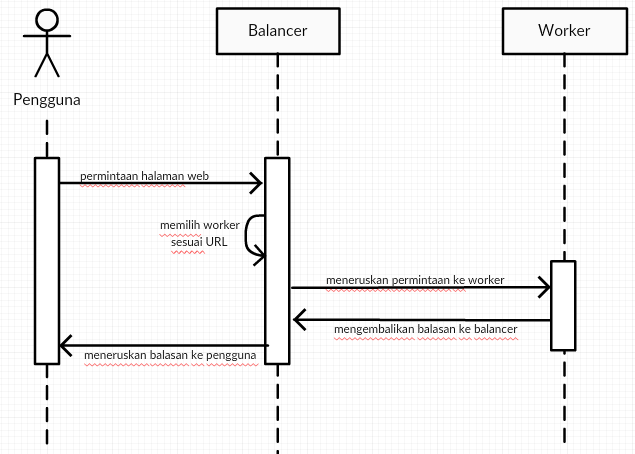
\includegraphics[width=\linewidth]{contoh_img/kerjabalancer}
			    	\caption{Diagram Interaksi antara Pengguna, Balancer dan Worker}
			    	\label{gambarKerjaBalancer}
			    \end{figure}
			
			\subsection{Deskripsi Rinci Worker}
				Worker bekerja sebagai pemberi layanan. Menunggu permintaan yang diteruskan dari balancer dan mengembalikan lagi ke balancer. Aplikasi berbasis web yang akan diakses pengguna dijalankan pada worker. Diagram arsitektur worker tertera pada Gambar \ref{gambarArsitekturWorker}
				
				\begin{figure}[] % h = pasti berada di bawah teks yang ada di atas
					\centering
					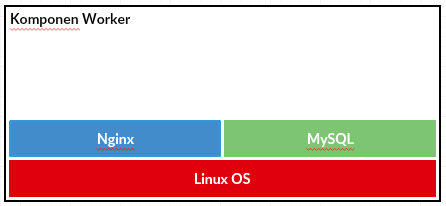
\includegraphics[width=\linewidth]{contoh_img/kompworker}
					\caption{Diagram Arsitektur Worker}
					\label{gambarArsitekturWorker}
				\end{figure}
				
				Di dalam sistem yang dibangun, peran \textit{worker} sudah digambarkan pada diagram proses yang tertera pada Gambar \ref{gambarKerjaBalancer}. Pengguna tidak dapat mengakses \textit{worker} secara langsung. Semua akses harus melalui \textit{balancer}. Walaupun sebenarnya semua aplikasi berada pada \textit{worker}.
			
			\subsection{Deskripsi Rinci Halaman Admin}
				Halaman ini hanya akan diakses oleh administrator sistem. Adanya halaman ini ditujukan untuk memudahkan admin dalam mengelola cluster dan mengelola URL yang tersimpan di dalam basis data. Digram arsitektur halaman admin tertera pada Gambar \ref{gambarArsitekturWeb}.
				
				\begin{figure}[] % h = pasti berada di bawah teks yang ada di atas
					\centering
					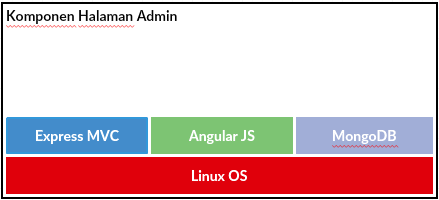
\includegraphics[width=\linewidth]{contoh_img/kompweb}
					\caption{Diagram Arsitektur Halaman Admin}
					\label{gambarArsitekturWeb}
				\end{figure}
				
				Express JS berperan dalam menangkap setiap rute yang diminta admin. Sementara Angular JS digunakan untuk menampilkan data sesuai dengan rute yang diminta admin. MongoDB yang digunakan dalam halaman admin sama dengan MongoDB yang digunakan oleh \textit{balancer}. Daftar rute yang dapat diakses admin tertera pada Tabel \ref{tabelRuteHalamanAdmin}.
				
				\begin{longtable}{|p{0.05\textwidth}|p{0.15\textwidth}|p{0.2\textwidth}|p{0.4\textwidth}|} % L = Rata kiri untuk setiap kolom, | = garis batas vertikal.
					
					% Kepala tabel, berulang di setiap halaman
					\caption{Rute pada Halaman Admin} \label{tabelRuteHalamanAdmin} \\
					\hline
					\textbf{No} & \textbf{Rute} & \textbf{Metode} & \textbf{Aksi} \\ \hline
					
					\endhead
					\endfoot
					\endlastfoot
					
					% Isi Tabel
					1 & / & GET, POST & Menampilkan status balancer dan operasi mengaktifkan/mematikan \textit{balancer}\\ \hline
					2 & /cluster & GET, POST & Mengelola \textit{worker} di dalam \textit{cluster} \\ \hline
					3 & /path & GET, POST & Mengelola rute pada aplikasi sesuai dengan \textit{cluster} \\ \hline

				\end{longtable}
				
			\subsection{Deskripsi Server Basis Data}
				Dalam menjalankan sebuah aplikasi yang menuntut kemampuan akses hingga banyak pengguna, banyak pengembang yang memisahkan antara server aplikasi dan server basis data. Aplikasi yang berjalan dalam server ini hanya MySQL sebagai basis data seperti yang tertera pada \ref{gambarArsitekturDB}.
			    
				\begin{figure}[h] % h = pasti berada di bawah teks yang ada di atas
					\centering
					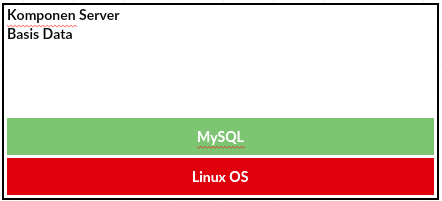
\includegraphics[width=\linewidth]{contoh_img/kompdb}
					\caption{Diagram Arsitektur Server Basis Data}
					\label{gambarArsitekturDB}
				\end{figure}


% vAB 4 BAB 4 BAB 4 BAB 4 BAB 4 BAB 4 BAB 4 BAB 4 BAB 4 BAB 4 BAB 4 BAB 4 BAB 4 BAB 4 BAB 4 BAB 4 BAB 4 BAB 4 BAB 4 BAB 4 BAB 4 BAB 4 BAB 4 BAB 4 BAB 4 BAB 4 BAB 4 BAB 4 BAB 4 BAB 4 BAB 4 BAB 4 BAB 4 BAB 4 BAB 4 BAB 4 BAB 4 BAB 4 BAB 4 BAB 4 BAB 4 BAB 4 BAB 4 BAB 4 BAB 4 BAB 4 BAB 4 BAB 4 BAB 4 BAB 4 BAB 4 BAB 4 BAB 4 BAB 4 BAB 4 BAB 4 BAB 4 BAB 4 BAB 4 BAB 4 BAB 4 BAB 4 BAB 4 BAB 4 BAB 4 BAB 4 BAB 4 BAB 4 BAB 4 BAB 4 BAB 4 BAB 4 BAB 4 BAB 4 BAB 4 BAB 4 BAB 4 BAB 4 BAB 4 BAB 4 BAB 4 BAB 4 BAB 4 BAB 4
		         
		         
	\chapter{Implementasi}
        Bab ini membahas implementasi sistem Load Balancing secara rinci. Pembahasan dilakukan secara rinci untuk setiap komponen yang ada yaitu: Balancer, Worker, Halaman Admin, dan Server Basis Data.
        
        \section{Lingkungan Implementasi}
	        Lingkungan implementasi dan pengembangan dilakukan menggunakan komputer dengan spesifikasi Intel(R) Core(TM) i3-2120 CPU @ 3.30GHz dengan memori 8 GB. Perangkat lunak yang digunakan dalam pengembangan adalah sebagai berikut :
	        \begin{itemize}
	        	\item Sistem Operasi Linux Ubuntu Server 14.04.01 LTS
	        	\item Desktop xfce4
	        	\item Editor teks vim
	        	\item Editor teks Sublime Text 2
	        	\item git versi 1.9.1 untuk pengolahan versi program
	        	\item NodeJS versi 4.2.3 untuk pengembangan aplikasi
	        	\item MongoDB versi 3.2.0 untuk basis data
	        	\item Express versi 4.13.1 untuk web server halaman admin
	        	\item Angular JS versi 1.5.0-beta.2 untuk pengolahan data pada halaman admin
	        	\item Nginx dan MySQL yang berjalan di \textit{worker} dan server basis data
	        	\item Paket \LaTeX untuk pembuatan tugas akhir
	        	\item Peramban \textit{web} Mozilla Firefox
	        \end{itemize}
	        
		\section{Rincian Implementasi Balancer}
		
			\textit{Balancer} dibangun dengan menggunakan Node JS, MongoDB dan beberapa paket yang diinstall secara terpisah. Paket-paket ini diinstall dengan menggunakan npm (\texttt{https://www.npmjs.com/}) yang memang digunakan sebagai \textit{command line} oleh Node JS. Pada sub bab ini akan dijelaskan implementasi mulai dari instalasi Node JS hingga \textit{balancer} siap digunakan.
			
			\subsection{Instalasi Node JS}
				Ada banyak cara untuk menginstall NodeJS ke dalam komputer, salah satunya melalui kode sumber yang dapat diunduh pada halaman \texttt{https://nodejs.org/en/download/}. Setelah diunduh berkas perlu diekstrak untuk melanjutkan instalasi. Di dalam folder hasil ekstraksi, terdapat berkas \texttt{README.md} yang berisi langkah untuk menginstall NodeJS ke komputer. Semua langkah dilakukan melalui \textit{command line} dan langkah installasinya adalah sebagai berikut
				
				\begin{itemize}
					\item Pindah ke folder dimana Node JS di ekstrak dengan perintah \texttt{cd \{\$pathdownload\}/node-v4.2.3/}.
					\item Di dalam folder jalankan perintah berikut secara berurutan \texttt{./configure}, \texttt{make}, \texttt{make install}.
					\item Jika terdapat pesan \textit{error} mengenai beberapa pustaka yang belum terinstall sebelumnya, jalankan perintah \texttt{sudo apt-get install -f}.
					\item Semua perintah dilakukan pada hak akses \textit{root}.
				\end{itemize}
				
				Untuk memastikan bahwa Node JS sudah berjalan dan siap digunakan, dijalankan perintah dan dihasilkan output seperti pada Gambar \ref{gambarCekNodeJS}.
				
				\begin{figure}[h] % h = pasti berada di bawah teks yang ada di atas
					\centering
					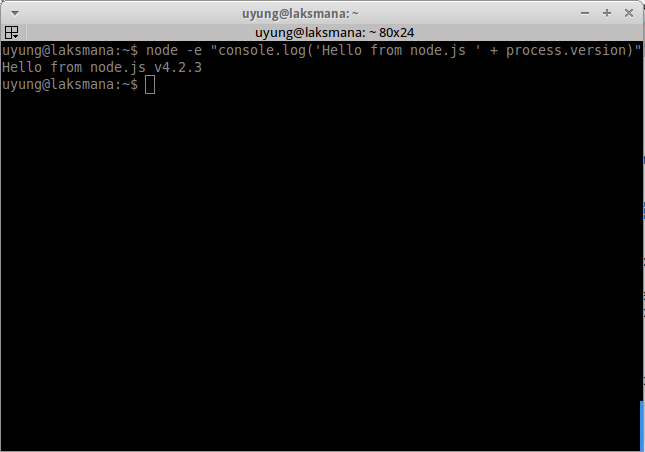
\includegraphics[width=\linewidth]{contoh_img/ceknodejs}
					\caption{Contoh Node JS Siap Digunakan}
					\label{gambarCekNodeJS}
				\end{figure}
			
			\subsection{Installasi MongoDB}
				MongoDB menyediakan repositori tersendiri untuk mengunduh MongoDB. Setelah terkoneksi dengan repositori yang dimiliki MongoDB, instalasi dapat berlanjut dengan menggunakan perintah \texttt{apt-get}. Berikut ini langkah-langkah instalasi MongoDB.
				
				\begin{itemize}
					\item Tambahkan \textit{public key} yang digunakan untuk manajemen paket pada sistem operasi dengan perintah \texttt{sudo apt-key adv --keyserver hkp://keyserver.ubuntu.com:80 --recv 7F0CEB10}.
					\item Buat file repositori untuk MongoDB pada sistem komputer dengan perintah \texttt{echo "deb http://repo.mongodb.org/apt/ubuntu trusty/mongodb-org/3.0 multiverse" | sudo tee /etc/apt/sources.list.d/mongodb-org-3.0.list}. Perintah ini disesuaikan dengan distro Linux yang digunakan.
					\item Perbaharui basis data manajemen paket dengan perintah \texttt{sudo apt-get update}.
					\item Install MongoDB ke komputer dengan perintah \texttt{sudo apt-get install -y mongodb-org}.
					\item Setelah instalasi selesai jalankan MongoDB dengan perintah \texttt{sudo service mongod start}.
					\item MongoDB siap digunakan dengan tampilan pada Gambar \ref{gambarCekMongoDB}.
					\begin{figure}[h] % h = pasti berada di bawah teks yang ada di atas
						\centering
						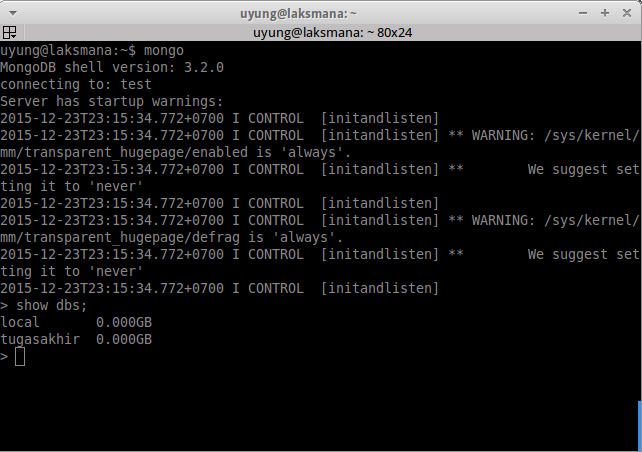
\includegraphics[width=\linewidth]{contoh_img/cekmongodb}
						\caption{Contoh MongoDB dan Daftar Database}
						\label{gambarCekMongoDB}
					\end{figure}
					
				\end{itemize}
				
				
			\subsection{Instalasi Paket}
			Seperti yang sudah dijelaskan sebelumnya, instalasi paket yang dibutuhkan menggunakan npm. Cara kerja npm ini hanya mengunduh paket untuk kebutuhan sistem, hanya saja beberapa paket bisa diinstall pada sistem operasi dan dapat digunakan pada \textit{command line}. 
			Untuk mengunduh paket yang dibutuhkan secara bersamaan, digunakan perintah \texttt{npm install}. Perintah ini akan membaca file \texttt{package.json} yang berisi daftar paket yang akan digunakan. Isi \texttt{package.json} untuk Tugas Akhir ini seperti pada Kode Sumber \ref{packageJson}

			\begin{lstlisting}[frame=single,tabsize=2,breaklines,caption={Isi Package.Json},label=packageJson]
{
	"name": "tugasakhir",
	"version": "1.0.0",
	"description": "Tugas Akhir ini berisi tentang load balancer dengan node JS",
	"dependencies": {
		"body-parser": "~1.13.2",
		"cookie-parser": "~1.3.5",
		"debug": "~2.2.0",
		"express": "~4.13.1",
		"express-session": "^1.7.6",
		"express-socket.io-session": "^1.3.1",
		"hbs": "~3.1.0",
		"helmet": "^0.10.0",
		"http-proxy": "^1.12.0",
		"moment": "~2.x.x",
		"mongoose": "^4.3.1",
		"morgan": "~1.6.1",
		"mysql": "~2.x.x",
		"net-ping": "^1.1.12",
		"node-sass-middleware": "0.8.0",
		"request": "^2.67.0",
		"serve-favicon": "~2.3.0",
		"socket.io": "~1.x.x"
	},
	"devDependencies": {},
	"scripts": {
		"test": "echo \"Error: no test specified\" && exit 1"
	},
	"repository": {
		"type": "git",
		"url": "git+https://github.com/bahrulhalimi/tugasakhir.git"
	},
	"keywords": [
		"balancer",
		"TA",
		"nodeJS"
	],
	"author": "Bahrul Halimi",
	"license": "ISC",
	"bugs": {
		"url": "https://github.com/bahrulhalimi/tugasakhir/issues"
	},
	"homepage": "https://github.com/bahrulhalimi/tugasakhir#readme"
}

				
			\end{lstlisting}
			
				Selain paket yang diinstall melalui perintah \texttt{npm install}, ada beberapa paket yang harus di install ke dalam sistem untuk bisa dipanggil melalui \textit{command line}. Salah satu paket yang digunakan dalam Tugas Akhir ini adalah \texttt{forever}. Paket ini harus di install ke komputer, sehingga dapat digunakan melalui \textit{command line}. Untuk menginstallnya digunakan perintah \texttt{sudo npm install forever -g}.
        
	        \subsection{Koneksi ke Basis Data}
		        Pada Tugas Akhir ini digunakan paket yang membantu untuk menghubungkan aplikasi dengan basis data yaitu paket \texttt{mongoose}. Untuk dapat terhubung dengan basis data, digunakan perintah \texttt{mongoose.connect('mongodb://127.0.0.1/tugasakhir')}
		        
		        Karena basis data yang digunakan MongoDB dan bersifat NoSQL, maka struktur tabel menjadi tidak wajib di deklarasikan di awal. Untuk selanjutnya dibuat model untuk mendeklarasikan setiap koneksi ke basis data, sesuai dengan tabel yang digunakan. Dalam MongoDB istilah tabel menjadi koleksi (\textit{collection}). Terdapat empat koleksi yang dibuat yaitu:
		        
		        \begin{itemize}
		        	\item aktivitas\_model, digunakan untuk mencatat setiap permintaan ke sistem.
		        	\item clusterinsert\_model, digunakan untuk mencatat daftar \textit{worker} di dalam \textit{cluster insert}.
		        	\item clusterview\_model, digunakan untuk mencatat daftar \textit{worker} di dalam \textit{cluster view}.
		        	\item path\_model, digunakan untuk mencatat daftar URL dan digolongkan ke dalam dua jenis, yaitu insert dan view.
		        \end{itemize}
		        
		        Kode program untuk setiap model tertera pada lampiran.
			
			\subsection{Implementasi Balancer}
				Algoritma berbasis konten diterapkan untuk menjalankan balancer. Algoritma ini hanya akan memilih \textit{worker} sesuai dengan \textit{cluster} yang aktif dan siap melayani permintaan. Daftar \textit{worker} yang dapat digunakan didapatkan dari basis data yang diakses dengan menggunakan model yang sudah di bahas pada sub-bab sebelumnya. Selanjutnya setiap permintaan akan dilempar ke \textit{worker} terpilih dan dilayani hingga permintaan selesai. Kode program untuk implementasi \textit{balancer} tertera pada Kode Program \ref{implemenBalancer}
				
				\begin{lstlisting}[frame=single,tabsize=2,breaklines,caption={Implementasi Algoritma Berbasis Konten pada Balancer},label=implemenBalancer]
blabla
				\end{lstlisting}
		
		\section{Rincian Implementasi Worker}
			Untuk melayani setiap permintaan dari pengguna, digunakan Nginx sebagai web server dan MySQL sebagai penyimpanan data dengan sistem operasi Ubuntu Server 14.04.03. \textit{Balancer} tidak menjalankan fungsi sebagai web server karena semua permintaan akan dilayani \textit{worker}. Untuk melakukan installasi kedua aplikasi tersebut digunakan perintah sebagai berikut:
			
			\begin{itemize}
				\item \texttt{sudo apt-get install nginx}. Perintah ini digunakan untuk instalasi Nginx ke dalam sistem operasi. Untuk dapat melayani halaman dinamis seperti PHP, diperlukan tambahan aplikasi lain yaitu php5-fpm. Untuk menginstalnya dijalankan perintah \texttt{sudo apt-get install php5-fpm}. 
				\item Berhubungan dengan php5-fpm, karena aplikasi yang akan dijalankan menggunakan kerangka kerja CodeIgniter, dibutuhkan paket lain yang dapat diinstall dengan perintah \texttt{sudo apt-get install php5-fpm php5-cgi php5-cli php5-mysql php5-curl php5-gd php5-idn php-pear php5-imagick php5-imap php5-mcrypt php5-memcache php5-mhash php5-pspell php5-recode php5-sqlite php5-tidy php5-xmlrpc php5-xsl} (https://bayultimate.wordpress.com/2012/05/08/daftar-paket-php-untuk-nginx/)
				\item Selanjutnya untuk menginstall MySQL digunakan perintah \texttt{sudo apt-get install mysql-server-5.5}
			\end{itemize}
			
			
			Terdapat empat \textit{worker} yang digunakan, dua server memiliki spesifikasi \textbf{kurang spek}
		
		\section{Implementasi Server Basis Data}
			Hanya ada satu aplikasi yang berjalan yaitu MySQL yang memberikan servis basis data kepada \textit{worker}. Konfigurasi lanjut dibutuhkan agar setiap \textit{worker} dapat menggunakan basis data yang ada. Salah satunya adalah alamat IP yang digunakan server harus dikenali lingkungan implementasi, dalam hal ini lingkungan di Laboratorium AJK. Selain alamat IP, konfigurasi lain yang dapat meningkatkan koneksi ke basis data juga diatur, dalam kasus ini variabel \texttt{max\_connections} dapat diperbesar nilainya untuk mendapatkan koneksi yang lebih banyak. Konfigurasi lengkap basis data tertera pada Kode Sumber
		    
		    \begin{lstlisting}[frame=single,tabsize=2,breaklines,caption={Konfigurasi MySQL untuk Server Basis Data},label=implemenDB]
#
# The MySQL database server configuration file.
#
# You can copy this to one of:
# - "/etc/mysql/my.cnf" to set global options,
# - "~/.my.cnf" to set user-specific options.
# 
# One can use all long options that the program supports.
# Run program with --help to get a list of available options and with
# --print-defaults to see which it would actually understand and use.
#
# For explanations see
# http://dev.mysql.com/doc/mysql/en/server-system-variables.html

# This will be passed to all mysql clients
# It has been reported that passwords should be enclosed with ticks/quotes
# escpecially if they contain "#" chars...
# Remember to edit /etc/mysql/debian.cnf when changing the socket location.
[client]
port		= 3306
socket		= /var/run/mysqld/mysqld.sock

# Here is entries for some specific programs
# The following values assume you have at least 32M ram

# This was formally known as [safe_mysqld]. Both versions are currently parsed.
[mysqld_safe]
socket		= /var/run/mysqld/mysqld.sock
nice		= 0

[mysqld]
#
# * Basic Settings
#
user		= mysql
pid-file	= /var/run/mysqld/mysqld.pid
socket		= /var/run/mysqld/mysqld.sock
port		= 3306
basedir		= /usr
datadir		= /var/lib/mysql
tmpdir		= /tmp
lc-messages-dir	= /usr/share/mysql
skip-external-locking
#
# Instead of skip-networking the default is now to listen only on
# localhost which is more compatible and is not less secure.
bind-address		= 10.151.36.205
#
# * Fine Tuning
#
key_buffer		= 64M
max_allowed_packet	= 16M
thread_stack		= 192K
thread_cache_size       = 8
# This replaces the startup script and checks MyISAM tables if needed
# the first time they are touched
myisam-recover         = BACKUP
max_connections        = 1024
#table_cache            = 64
#thread_concurrency     = 10
#
# * Query Cache Configuration
#
query_cache_limit	= 10M
query_cache_size        = 64M
#
# * Logging and Replication
#
# Both location gets rotated by the cronjob.
# Be aware that this log type is a performance killer.
# As of 5.1 you can enable the log at runtime!
#general_log_file        = /var/log/mysql/mysql.log
#general_log             = 1
#
# Error logging goes to syslog due to /etc/mysql/conf.d/mysqld_safe_syslog.cnf.
#
# Here you can see queries with especially long duration
#log_slow_queries	= /var/log/mysql/mysql-slow.log
#long_query_time = 2
#log-queries-not-using-indexes
#
# The following can be used as easy to replay backup logs or for replication.
# note: if you are setting up a replication slave, see README.Debian about
#       other settings you may need to change.
#server-id		= 1
#log_bin			= /var/log/mysql/mysql-bin.log
expire_logs_days	= 10
max_binlog_size         = 100M
#binlog_do_db		= include_database_name
#binlog_ignore_db	= include_database_name
#
# * InnoDB
#
# InnoDB is enabled by default with a 10MB datafile in /var/lib/mysql/.
# Read the manual for more InnoDB related options. There are many!
#
# * Security Features
#
# Read the manual, too, if you want chroot!
# chroot = /var/lib/mysql/
#
# For generating SSL certificates I recommend the OpenSSL GUI "tinyca".
#
# ssl-ca=/etc/mysql/cacert.pem
# ssl-cert=/etc/mysql/server-cert.pem
# ssl-key=/etc/mysql/server-key.pem



[mysqldump]
quick
quote-names
max_allowed_packet	= 16M

[mysql]
#no-auto-rehash	# faster start of mysql but no tab completition

[isamchk]
key_buffer		= 16M

#
# * IMPORTANT: Additional settings that can override those from this file!
#   The files must end with '.cnf', otherwise they'll be ignored.
#
!includedir /etc/mysql/conf.d/
		    
		    \end{lstlisting}
		
		\section{Implementasi Halaman Admin}

\appendix % Halaman lampiran, dengan judul LAMPIRAN X

\backmatter % Lampiran tanpa judul LAMPIRAN X, biasanya untuk BIODATA PENULIS
\end{document}
